\documentclass[aspectratio=169]{beamer}

\setlength{\headheight}{26pt}

% Packages
\usepackage[left=25mm, right=25mm, top=35mm, bottom=25mm]{geometry} % defines whitespaces on the edges
\usepackage[bottom, hang]{footmisc}
\usepackage{hyperref}             % for \nameref and cite
\usepackage{footnotebackref}      % used for getting back from the footnote to the main text
\usepackage{enumitem}
\usepackage{graphicx}
\usepackage{fancyhdr}
\usepackage{lastpage}
\usepackage[export]{adjustbox}
\usepackage{float}
\usepackage[ngerman]{babel}
\usepackage[ngerman]{datetime}
\usepackage{apacite}
\usepackage[utf8]{inputenc}
\usepackage{listings}
\usepackage{xcolor}
\usepackage{pdfpages}
\usepackage{url}
\usepackage{outlines}
\usepackage{tocloft}
\usepackage[utf8]{inputenc}
\usepackage{amsmath}
\usepackage{mathtools}
\usepackage[acronym]{glossaries}
\usepackage{titlesec}             % for \titleformat
\usepackage{textcomp}             % for \degree sign
\usepackage{gensymb}              % for \degree sign
\usepackage{csvsimple}            % for using csv-files for tables
\usepackage{lscape}               % for landscape mode
\usepackage{parskip}              % inserts space after paragraph automatically
\usepackage{svg}                  % used to include svg with the help of inkscape which converts svg to pdf
\usepackage{wasysym}              % for \diameter symbol
\usepackage{xfrac}                % for \sfrac

\frenchspacing  % Use same space size between words and between sentences

% change section titles' font size
\titleformat*{\section}{\huge\bfseries}
\titleformat*{\subsection}{\LARGE\bfseries}
\titleformat*{\subsubsection}{\Large\bfseries}
\titleformat{\paragraph}[hang]{\large\bfseries}{\theparagraph}{1em}{}
\titleformat{\subparagraph}[hang]{\normalsize\bfseries}{\thesubparagraph}{1em}{}

\definecolor{codegreen}{rgb}{0,0.6,0}
\definecolor{codegray}{rgb}{0.5,0.5,0.5}
\definecolor{codepurple}{rgb}{0.58,0,0.82}
\definecolor{codeorange}{rgb}{1,0.5,0.15}
\definecolor{backcolour}{rgb}{0.9,0.9,0.9}

\lstdefinestyle{mystyle}{
    backgroundcolor=\color{backcolour},
    commentstyle=\color{codegreen},
    keywordstyle=\color{magenta},
    numberstyle=\tiny\color{codegray},
    stringstyle=\color{codepurple},
    basicstyle=\ttfamily\footnotesize,
    breakatwhitespace=false,
    breaklines=true,
    captionpos=b,
    keepspaces=true,
    numbers=left,
    numbersep=5pt,
    showspaces=false,
    showstringspaces=false,
    showtabs=false,
    tabsize=4
}
\lstset{style=mystyle}

\lstset{
    literate={~} {$\sim$}{1}
}

\lstset{%
    breaklines=true,
    breakatwhitespace=true,
}

\DeclarePairedDelimiter\abs{\lvert}{\rvert} % make scalable absolute stripes
\DeclarePairedDelimiter\parenth{(}{)} % make scalable parentheses

\let\phi\varphi{} % change style of \phi sign

\setlength{\parindent}{0mm} % disable paragraph indent

\newdateformat{mydate}{\THEDAY{. }\monthnamengerman[\THEMONTH] \THEYEAR}

\renewcommand{\listfigurename}{}
\renewcommand\contentsname{Inhaltsverzeichnis}
\renewcommand\lstlistingname{Code}

\makeglossaries{}

% Header/Footer Setting
\setlength\footnotemargin{15pt}
\pagestyle{fancy}
\fancyhf{}
\renewcommand{\footrulewidth}{0.4pt} % footer line
\rhead{\textbf{\vUniversity}\\\vModule}
\lhead{\textbf{\vTitle}\\
    Projektarbeit}
\lfoot{\vAuthorFirstName{} \vAuthorLastName}
\cfoot{\mydate\today}
\rfoot{S.~\thepage~/~\pageref{LastPage}}

% Redefine the plain page style, otherwise there is no header and footer for chapter pages
\fancypagestyle{plain}{%
    \fancyhf{}
    \renewcommand{\footrulewidth}{0.4pt} % footer line
    \rhead{\textbf{\vUniversity}\\\vModule}
    \lhead{\textbf{\vTitle}\\
        Projektarbeit}
    \lfoot{\vAuthorFirstName{} \vAuthorLastName}
    \cfoot{\mydate\today}
    \rfoot{S.~\thepage~/~\pageref{LastPage}}
}

\bibliographystyle{apacite}

% Settings for the equation list
\newcommand{\listequationsname}{}
\newlistof{myequations}{equ}{\listequationsname}
\renewcommand{\cftmyequationsaftersnum}{\hfill}
\renewcommand{\cftmyequationspresnum}{\hfill}
\setlength{\cftmyequationsnumwidth}{3.5em}
\newcommand{\myequations}[1]{%
\addcontentsline{equ}{myequations}{\protect\numberline{\theequation}#1}\par}

\newcommand{\mytable}[4]
{
    \centering
    \begin{tabular}{#1}\hline%
        #2 \\ \hline
        \csvreader[
            separator=semicolon,
            head to column names,
            late after line=\\,
        ]{#4}{}{#3}
        \hline
    \end{tabular}
}


% Variables
\title{DIY Optische ToF Distanzmessung}
\author{Matthias Schär, Timon Burkard}
\institute{OST -- Ostschweizer Fachhochschule}
\date{24.01.2025}
\newcommand{\vModule}{CAS Sensorik und Sensor Signal Conditioning}

\begin{document}

{
    \setbeamertemplate{headline}{}
    \setbeamertemplate{footline}{}
    \begin{frame}
        \titlepage{}
    \end{frame}
}
\setlistspacing{1}{2ex}


%%%%%%%%%%%%%%%%%%%%%% CONTENT START %%%%%%%%%%%%%%%%%%%%%%

\begin{frame}{Inhaltsverzeichnis}
    \tableofcontents
\end{frame}


\section{Beispiel Kapitel 1}

\subsection{Unterkapitel Bilder}

\begin{frame}{Beispiel Frame}
    \begin{itemize}
        \item Aufzählung Element 1
        \item<2-> Aufzählung Element 2
        \begin{itemize}
            \item Unterelement 1
            \item Unterelement 2
        \end{itemize}
    \end{itemize}

    \onslide<3->
    {
        \begin{figure}
            \includegraphics[width=0.38\textwidth]{graphics/example.jpg}
            \sidecaption{\cite{pixabay2018pcb}}
        \end{figure}
    }
\end{frame}

\begin{frame}{Annotation eines Bildes}
    \begin{itemize}
        \item Bild highlighted:
    \end{itemize}

    \onslide<2->
    {
        \begin{figure}
            \includegraphics[width=0.53\textwidth]{graphics/example.jpg}
        \end{figure}
    }

    \onslide<3->
    {
        \highlight{4.4, 2.8}{6.9, 1.1}
    }
\end{frame}

\subsection{Unterkapitel weitere Grafiken}

\begin{frame}{draw.io Diagramme}
    \begin{itemize}
        \item Es können \lstinline|draw.io| Diagramme eingefügt werden:
    \end{itemize}

    \onslide<2->
    {
        \begin{figure}[H]
            \centering
            \includegraphics[width=0.9\textwidth]{diagrams/example.pdf}
        \end{figure}
    }
\end{frame}

\begin{frame}{PDF Seiten}
    \begin{figure}[H]
        \centering
        \fbox{\includegraphics[page=49,height=0.76\textheight]{documents/example.pdf}}
        \sidecaption{\cite{embedded2019marketsstudy}}
    \end{figure}
\end{frame}

\begin{frame}{SVG}
    \begin{itemize}
        \item Es können \lstinline|SVG| Bilder eingefügt werden:
    \end{itemize}

    \onslide<2->
    {
        \begin{figure}
            \includesvg[width=0.6\textwidth]{graphics/example.svg}
            \sidecaption{\cite{wikipedia2023mikrofon}}
        \end{figure}
    }
\end{frame}

\begin{frame}{GIF}
    \begin{itemize}
        \item Es können \lstinline|GIF| Animationen eingefügt werden:
    \end{itemize}

    \begin{figure}
        \animategraphics[width=0.3\textwidth]{10}{animations/fledermaus-}{0}{14}
        \caption{\cite{wikipedia2023laufzeitmessung}}
    \end{figure}
\end{frame}

\section{Beispiel Kapitel 2}

\begin{frame}{Zwei Spalten}
    \begin{columns}
        \column{0.5\textwidth}
            Etwas Text auf der linken Seite.\\~\\

            Lorem ipsum dolor sit amet, consectetur adipiscing elit, sed do eiusmod tempor incididunt ut labore et dolore magna aliqua. Ut enim ad minim veniam, quis nostrud exercitation ullamco laboris nisi ut aliquip ex ea commodo consequat.\cite{lipsum2022lorem}
        \column{0.5\textwidth}
            Etwas Text auf der rechten Seite.\\~\\

            Lorem ipsum dolor sit amet, consectetur adipiscing elit, sed do eiusmod tempor incididunt ut labore et dolore magna aliqua. Ut enim ad minim veniam, quis nostrud exercitation ullamco laboris nisi ut aliquip ex ea commodo consequat.\cite{lipsum2022lorem}
    \end{columns}
\end{frame}

\begin{frame}{Frage stellen}
    \question{Was ist Unterschiede zu 8bit AVR\@?}
\end{frame}

\begin{frame}{Bitte beachten}
    \attention{Nie einen Kurzschluss verursachen!}
\end{frame}

\begin{frame}{Übung}
    \exercise[https://gitlab.com/hfie-bm_ed3/hs22]{Arbeitsblatt01}
\end{frame}

\section{Beispiel Kapitel 3}

\begin{frame}{Erstes Beispiel in C}
    \lstinputlisting{sourcecode/example1.c}
\end{frame}

\begin{frame}{Zweites Beispiel in C}
    \begin{itemize}
        \item Es kann auch durch den Code gesteppt werden (highlight vs.\ grey-out):
    \end{itemize}

    \onslide<2->
    {
        \only<-2>{\codehighlight{C}{1}{99}{sourcecode/example2.c}}
        \only<3>{\codehighlight{C}{1}{1}{sourcecode/example2.c}}
        \only<4>{\codehighlight{C}{3}{4}{sourcecode/example2.c}}
        \only<5>{\codehighlight{C}{6}{7}{sourcecode/example2.c}}
        \only<6>{\codehighlight{C}{9}{15}{sourcecode/example2.c}}
        \only<7>{\codehighlight{C}{12}{12}{sourcecode/example2.c}}
        \only<8>{\codehighlight{C}{13}{13}{sourcecode/example2.c}}
        \only<9>{\codehighlight{C}{14}{14}{sourcecode/example2.c}}
    }

\end{frame}

\section{Beispiel Kapitel 4}

\begin{frame}{Tabulatoren}
    \begin{itemize}
        \item Es können Tabulatoren verwendet werden:
        \begin{itemize}
            \item Erstens:  \tabto{45pt} Das ist das Erste
            \item Zweitens: \tabto{45pt} Das ist das Zweite
            \item Drittens: \tabto{45pt} Das ist das Dritte
        \end{itemize}
    \end{itemize}
\end{frame}

\begin{frame}{Tabelle}
    \begin{table}[H]
        \centering
        \renewcommand{\arraystretch}{1.4}
        \begin{tabular}{|l|l|l|}\hline%
        \bfseries Datentyp & \bfseries Grösse & \bfseries Beschreibung \\ \hline
        \csvreader[
            separator=semicolon,
            head to column names,
            late after line=\\ \hline,
        ]{tables/example.csv}{}{\datentyp & \groesse & \beschreibung}
        \end{tabular}
    \end{table}
\end{frame}

\begin{frame}{Formeln}
    \begin{itemize}
        \item Es können Formeln eingefügt werden:
    \end{itemize}

    \begin{equation*}
        \begin{split}
            y = \parenth*{\frac{x}{Messbereich}} \cdot 2^A \\
        \end{split}
    \end{equation*}

    \onslide<2->
    {
        \begin{itemize}
            \item Um mehrere Formeln ausgerichtet darzustellen:
        \end{itemize}

        \begin{equation*}
            \begin{split}
                s & = \cos(\omega_d \cdot t) + j \cdot \sin(\omega_d \cdot t) \\
                & = e^{j \cdot \omega_d \cdot t}
            \end{split}
        \end{equation*}
    }
\end{frame}

%%%%%%%%%%%%%%%%%%%%%% CONTENT END %%%%%%%%%%%%%%%%%%%%%%

\miniframesoff

\questions{}

\begin{frame}[allowframebreaks]{Quellen}
    \nocite{*} % add all sources to bibliography not just the cited ones
    \bibliographystyle{unsrtnat}
    {\scriptsize \bibliography{./references.bib}}
\end{frame}


\end{document}
